\documentclass[11pt]{report}
\usepackage{mathtools}
\usepackage{amsmath}
\usepackage{amssymb}
\usepackage{amsfonts}
\usepackage{amsthm}
\usepackage{xcolor}
\usepackage{graphicx}
\usepackage[top=2.0cm,bottom=2.0cm,left=2.5cm,right=2.5cm]{geometry}
\usepackage{tikz}
\usepackage{float}
\usepackage{multicol}
\usepackage{pgfplots}
\usepackage{lastpage}
\usepackage{siunitx}
\usepackage{xspace}
\usepackage[labelfont=bf]{caption}
\usepackage[hidelinks, urlcolor=blue, linkcolor=blue, colorlinks=true]{hyperref}
\usepackage[capitalize,noabbrev]{cleveref}
\usepackage[absolute]{textpos}
\usepackage{systeme}

\newcommand{\R}{\mathbb{R}}
\newcommand{\C}{\mathbb{C}}
%% define course title
\newcommand{\course}{MAT185}
\newcommand{\assignmenttitle}{Assignment 1}

%% header and footer
\firstpageheader{}{}{\textbf{{\color{red} Due:} 10:00pm, Tuesday Jan. 21, 2025}}
\firstpageheadrule
\runningheader{}{Page~\thepage~of~\numpages}{\course~--~\assignmenttitle}
\footer{}{}{}

\setlength\parindent{0pt} % no indentation in document

%% formats exam class
\qformat{\textbf{Question \thequestiontitle:}\hfill} % title of question 
\boxedpoints
\pointpoints{mark}{marks}
\pointsinrightmargin
\hpword{Marks:}
\hsword{Your score:}
\unframedsolutions
\totalformat{\boxed{\textnormal{\totalpoints~\if\totalpoints1 mark\else marks\fi}}}
\definecolor{SolutionColor}{rgb}{0,0,1}
\renewcommand{\solutiontitle}{}
\AtBeginEnvironment{solution}{\color{blue}}

% %correct choices in solution
\CorrectChoiceEmphasis{\rm}
\checkedchar{\tikz\draw[blue,fill=blue] (0,0) circle (1ex);}

% % increase distance between checkbox items
\renewcommand{\checkboxeshook}{\setlength{\itemsep}{6pt}}

%% distance between questions and parts
\renewcommand{\questionshook}{\setlength{\parsep}{10pt}}
\renewcommand{\partshook}{\setlength{\parsep}{15pt}}

%% define arrows in text
\newcommand{\arrow}{$\rightarrow$\xspace}
\newcommand{\Arrow}{$\Rightarrow$\xspace}

% % math notation:
%\veccol{1}{2}{3}
\newcommand{\veccol}[3]{
    \begin{bmatrix}
        #1\\
        #2\\
        #3\\
    \end{bmatrix}}
  
%\vecrow{1}{2}{3}
\newcommand{\vecrow}[3]{\left[#1~#2~ #3\right]}

%\matrixTwo{1}{2}{3}{4}
\newcommand{\matrixTwo}[4]{\left[\begin{array}{cc}#1&#2\\#3&#4\end{array}\right]}

% \matrixThree{1}{2}{3}{4}{5}{6}{7}{8}{9}
\newcommand{\matrixThree}[9]{\left[\begin{array}{ccc}#1&#2&#3\\#4&#5&#6\\#7&#8&#9\end{array}\right]}

%\matrixCorner{1}{2}{3}{4}
\newcommand{\matrixCorner}[4]{\left[\begin{array}{ccc}#1& \cdots&#2\\ \vdots & \ddots & \vdots\\#3&
      \cdots&#4\end{array}\right]}

% \nR
\newcommand{\nR}{{}^{n}\mathbb{R}}
% \Rn
\newcommand{\Rn}{\mathbb{R}^{n}}
% \nRn
\newcommand{\nRn}{{}^{n}\mathbb{R}^{n}}
% \nRm
\newcommand{\nRm}{{}^{n}\mathbb{R}^{m}}
% \nRm
\newcommand{\mRn}{{}^{m}\mathbb{R}^{n}}
% \mRm
\newcommand{\mRm}{{}^{m}\mathbb{R}^{m}}        

% \u
\renewcommand{\u}{{\bf u}}      
% \v
\renewcommand{\v}{{\bf v}}      
% \w
\newcommand{\w}{{\bf w}}    
% \V
\newcommand{\V}{{\bf V}}                   
       
%% define abbreviations
\newcommand{\row}{\operatorname{row}\,}
\newcommand{\col}{\operatorname{col}\,}
\renewcommand{\dim}{\operatorname{dim}\,}
\renewcommand{\span}{\operatorname{span}\,}
\newcommand{\rank}{\operatorname{rank}\,}
\renewcommand{\ker}{\operatorname{ker}\,}
\newcommand{\nul}{\operatorname{null}\,}
\renewcommand{\det}{\operatorname{det}\,}
\newcommand{\adj}{\operatorname{adj}\,}

\usepackage{xcolor}
% Sean's original colours:
%\definecolor{dkrgreen}{rgb}{0.1, 0.4, 0.3} 
\definecolor{dkrgreen}{HTML}{009988} % this is the color-blind friendly teal from below
%\definecolor{dkred}{rgb}{0.8, 0.05, 0.05} 
\definecolor{dkred}{HTML}{EE3377}  % this is the colour-blind friendly magenta from below
%\definecolor{orange}{rgb}{0.8, 0.33, 0.0}
%\definecolor{goldenrod}{rgb}{0.85, 0.65, 0.13}
\definecolor{blue}{HTML}{1965B0} % this is the colour-blind friendly blue from below
%
% colour-blind-friendly colours from https://personal.sron.nl/~pault/
\definecolor{tolBlue}{HTML}{1965B0}
\definecolor{tolMedBlue}{HTML}{5289C7}
\definecolor{tolLightBlue}{HTML}{7BAFDE} 
\definecolor{tolRed}{HTML}{E8601C} 
\definecolor{tolYellow}{HTML}{F6C141}
\definecolor{tolTeal}{HTML}{009988}
%\definecolor{tolBlue}{HTML}{0077BB} 
\definecolor{tolCyan}{HTML}{33BBEE}
\definecolor{tolTeal}{HTML}{009988} 
\definecolor{tolOrange}{HTML}{EE7733} 
%\definecolor{tolRed}{HTML}{CC3311} 
\definecolor{tolMagenta}{HTML}{EE3377} 
\definecolor{tolGrey}{HTML}{BBBBBB}

%%% This command makes a framed box of a chosen height.
\newcommand{\makenonemptybox}[2]{%
\par\nobreak\vspace{\ht\strutbox}\noindent
\setlength{\fboxrule}{0pt} % set this to 0pt to make invisible
\fbox{%
\parbox[c][#1][t]{\dimexpr\linewidth-2\fboxsep}{
  \hrule width \hsize height 0pt
  \vspace{-0.6cm}
  \color{SolutionColor}#2\color{black}
 }%
}%
}


\begin{document}
\thispagestyle{empty}
{\LARGE \bf AER 210 Lecture Notes}\\
{\large Hei Shing Cheung}\\
Vector Calculus \& Fluid Mechanics, Fall 2025 \hfill AER210\\
\\
The up-to-date version of this document can be found at \url{https://github.com/HaysonC/skulenotes}\\

\chapter{Vector Calculus}

% set section counter from 15 
\setcounter{section}{13}
\paragraph{Note} the section numbering is based on Stewart's book.

\section{Partial Derivatives}
\subsection{Taylor Series for Multivariable Functions}
\paragraph{Continuing from Calc II} We consider Taylor series of multivariable functions, and we would need to consider partial derivatives.

\begin{shaded}
    \subsubsection{Review. Taylor Series for Single Variable Functions}
    Let $f(x)$ be a function that is infinitely differentiable at $x = a$. The Taylor series of $f(x)$ about the point $x = a$ is given by:
    \begin{equation}
        f(x) = f(a) + f'(a)(x-a) + \frac{f''(a)}{2!}(x-a)^2 + \frac{f'''(a)}{3!}(x-a)^3 + \cdots = \sum_{n=0}^{\infty} \frac{f^{(n)}(a)}{n!} (x-a)^n
    \end{equation}

    Also, consider the taylor approximation of $f(x + \Delta x)$ about $x$: 
    \begin{equation}
        f(x + \Delta x) = f(x) + f'(x)\Delta x + \frac{f''(x)}{2!}(\Delta x)^2 + \frac{f'''(x)}{3!}(\Delta x)^3 + \cdots = \sum_{n=0}^{\infty} \frac{f^{(n)}(x)}{n!} (\Delta x)^n
    \end{equation}
\end{shaded}
\begin{definition}[Taylor Series for Multivariable Functions]
    Let $f(x,y)$ be a function that is infinitely differentiable at the point $(a,b)$. Consider the increment $\Delta x$ in the $x$-direction and $\Delta y$ in the $y$-direction centred at $(x_0,y_0)$. We have the following parametric equations:
    $$
        \begin{cases}
            x = x_0 + \Delta x t \\
            y = y_0 + \Delta y t
        \end{cases} \quad t \in [0,1]
    $$
    Define a new function $g(t) = f(x_0 + \Delta x t, y_0 + \Delta y t)$, which is a single-variable function in terms of $t$. We can then apply the Taylor series for single-variable functions to $g(t)$ about $t = 0$:
    $$
        g(t) = g(0) + g'(0)t + \frac{g''(0)}{2!}t^2 + \frac{g'''(0)}{3!}t^3 + \cdots = \sum_{n=0}^{\infty} \frac{g^{(n)}(0)}{n!} t^n
    $$
    Using the chain rule, we can compute the taylor series of $f(x,y)$ about the point $(x_0,y_0)$:
    \begin{align}
        f(x_0 + \Delta x, y_0 + \Delta y) &= f(x_0,y_0) + \left( \frac{\partial f}{\partial x} \Delta x + \frac{\partial f}{\partial y} \Delta y \right) + \nonumber \\
        &\quad \frac{1}{2!} \left( \frac{\partial^2 f}{\partial x^2} (\Delta x)^2 + 2\frac{\partial^2 f}{\partial x \partial y} \Delta x \Delta y + \frac{\partial^2 f}{\partial y^2} (\Delta y)^2 \right) + \cdots \\
        &= f(x_0,y_0) + \sum_{n=1}^{\infty} \sum_{k=0}^n \frac{1}{k!(n-k)!} \frac{\partial^n f}{\partial x^k \partial y^{n-k}} (\Delta x)^k (\Delta y)^{n-k}
    \end{align}
    Or equivalently, we can write:
    \begin{equation}
        f(x,y) = f(x_0,y_0) + \sum_{n=1}^{\infty} \sum_{k=0}^n \frac{1}{k!(n-k)!} \frac{\partial^n f}{\partial x^k \partial y^{n-k}} (x - x_0)^k (y - y_0)^{n-k}
    \end{equation}
    We could also use the fact:
    $$
        \frac{1}{k!(n-k)!} = \frac{1}{n!} \binom{n}{k}
    $$
    we rewrite the above equations, such that we can use the pascal's triangle to help us remember the coefficients:
    \begin{equation}
        f(x,y) = f(x_0,y_0) + \sum_{n=1}^{\infty} \frac{1}{n!} \sum_{k=0}^n \binom{n}{k} \frac{\partial^n f}{\partial x^k \partial y^{n-k}} (x - x_0)^k (y - y_0)^{n-k}
    \end{equation}

\end{definition}
\section{Multiple Integrals}
\begin{definition}[Double Integral]
    Let $f(x,y)$ be a function defined on a closed and bounded region $R$ in the $xy$-plane. The double integral of $f$ over $R$ is denoted by
    \begin{equation}
        \iint_R f(x,y) \, dA = \iint_R f(x,y) \, dA
    \end{equation}
    where $dA$ represents an infinitesimal area element in the region $R$. The double integral can be interpreted as the volume under the surface defined by $z = f(x,y)$ over the region $R$.
\end{definition}

\subsection{Double Integrals in a Rectangular Region}

 By the point of seeing this note, you should be familiar with the simple case of rectangular, simple cases are provided as examples:

\begin{example}
    Find the area under the quadric surface $z = 16 - x^2 - y^2$ over the square region $R = \{ (x,y) \mid 0 \le x \le 2, 0 \le y \le 2\}$.

    \textbf{Note} We would have to ensure that the surface is above the $xy$-plane in the region of interest, which is true in this case.

    We can set up the double integral as follows:
    $$
        \iint_R (16 - x^2 - y^2) \, dA = \int_0^2 \int_0^2 (16 - x^2
        - y^2) \, dy \, dx
    $$
    First, we integrate with respect to $y$:
    $$
        \int_0^2 (16 - x^2 - y^2) \, dy = \left[ 16y - x^2y - \frac{y^3}{3} \right]_0^2 = 32 - 2x^2 - \frac{8}{3} = \frac{88}{3} - 2x^2
    $$
    Next, we integrate with respect to $x$:
    $$
        \int_0^2 \left( \frac{88}{3} - 2x^2 \right) \, dx = \left[ \frac{88}{3}x - \frac{2x^3}{3} \right]_0^2 = \frac{176}{3} - \frac{16}{3} = \frac{160}{3}
    $$
    Therefore, the area under the surface is $\frac{160}{3}$.

\end{example}

\begin{example}
    Evaluate the double integral of $f(x,y) = x - 3y^2$ over the rectangular region $R = \{ (x,y) \mid 0 \le x \le 2, 1 \le y \le 2\}$.

    We can set up the double integral as follows:
    $$
        \iint_R (x - 3y^2) \, dA = \int_0^2 \int_1^2 (x - 3y^2) \, dy \, dx
    $$
    First, we integrate with respect to $y$:
    $$
        \int_1^2 (x - 3y^2) \, dy = \left[ xy - y^3 \right]_1^2 = 2x - 8 - (x - 1) = x - 7
    $$
    Next, we integrate with respect to $x$:
    $$
        \int_0^2 (x - 7) \, dx = \left[ \frac{x^2}{2} - 7x \right]_0^2 = \left( 2 - 14 \right) - 0 = -12
    $$
    Therefore, the value of the double integral is $-12$.
\end{example}

\begin{theorem}
    If the integrand function $f(x,y)$ is seperable, i.e., $f(x,y) = g(x)h(y)$, then the double integral can be computed as follows:
    \begin{equation}
        \iint_R f(x,y) \, dA = \left( \int_a^b g(x) \, dx \right) \left( \int_c^d h(y) \, dy \right)
    \end{equation}
    where $R = \{ (x,y) \mid a \le x \le b, c \le y \le d \}$.
\end{theorem}
\begin{proof}
    \textbf{Sketch:} $h(y)$ is a constant when integrating with respect to $x$, and vice versa.
\end{proof}

\begin{example}
    Let $f(x,y) = \sin{x} \cos{y}$ and $R = \{ (x,y) \mid 0 \le x \le \frac{\pi}{2}, 0 \le y \le \frac{\pi}{2} \}$. Evaluate the double integral $\iint_R f(x,y) \, dA$.

    Since $f(x,y)$ is seperable, we can write:
    $$
        \iint_R f(x,y) \, dA = \left( \int_0^{\frac{\pi}{2}} \sin{x} \, dx \right) \left( \int_0^{\frac{\pi}{2}} \cos{y} \, dy \right)
    $$
    Evaluating each integral separately gives 1 for both, so the final result is: $1 \times 1 = 1$.
\end{example}
\subsection{Double Integrals in General Regions}
\paragraph{Types of Regions} When the region $R$ is not rectangular, we can still compute the double integral by expressing the region in terms of inequalities. There are three common types of regions:
\begin{definition}[Type I Region]
    A region $R$ is called a Type I region if it can be described by the inequalities:
    $$
        a \le x \le b, \quad g_1(x) \le y \le g_2(x)
    $$
    where $g_1(x)$ and $g_2(x)$ are continuous functions on the interval $[a,b]$. Then, to evaluate the double integral over a Type I region for a continuous function $f(x,y)$, we set up the integral as follows:

    \begin{equation}
        \iint_R f(x,y) \, dA = \int_a^b \int_{g_1(x)}^{g_2(x)} f(x,y) \, dy \, dx
    \end{equation}

    \textbf{Integral Order:} Integrate with respect to $y$ first, then $x$.

    \textbf{Intuition:} As we traverse the outer part ($x$), we are summing up vertical slices (in $y$), and the bounds of those slices depend on $x$ and changes.
\end{definition}

\begin{definition}[Type II Region]
    Type II reigion is similar to Type I, but the roles of $x$ and $y$ are swapped. A region $R$ is called a Type II region if it can be described by the inequalities:
    $$
        c \le y \le d, \quad h_1(y) \le x \le h_2(y)
    $$
    where $h_1(y)$ and $h_2(y)$ are continuous functions on the interval $[c,d]$. Then, to evaluate the double integral over a Type II region for a continuous function $f(x,y)$, we set up the integral as follows: 
    \begin{equation}
        \iint_R f(x,y) \, dA = \int_c^d \int_{h_1(y)}^{h_2(y)} f(x,y) \, dx \, dy
    \end{equation}

    The integral order and intuition is mirrored from Type I, but we are summing up horizontal slices (in $x$), and the bounds of those slices depend on $y$ and changes.
\end{definition}

\begin{definition}[Type III Region]
    A region $R$ is called a Type III region if it can be described as the union of a finite number of Type I and Type II regions. To evaluate the double integral over a Type III region for a continuous function $f(x,y)$, we can break down the integral into separate integrals over each Type I or Type II subregion and sum them up:
    \begin{equation}
        \iint_R f(x,y) \, dA = \sum_{i=1}^n \iint_{R_i} f(x,y) \, dA
    \end{equation}
    where each $R_i$ is either a Type I or Type II region. And that:
    $$
        \bigcup_{i=1}^n R_i = R \quad \text{and} \quad R_i \cap R_j = \emptyset \text{ for } i \neq j
    $$
    This approach allows us to handle more complex regions by breaking them down into simpler parts.
\end{definition}

\begin{example}
    Find the volume of the solid that lies under the paraboloid $z = f(x,y) = x^2 + y^2$ and above the region $R$ bounded
     by $y = 2x$ and $y = x^2$.

     First, you would sketch the region to understand its shape and boundaries at Figure \ref{fig:region}.

    \begin{figure}[h]
        \centering
        \begin{tikzpicture}
            \begin{axis}[
                axis lines = middle,
                xlabel = $x$,
                ylabel = $y$,
                xmin = -1, xmax = 3,
                ymin = -1, ymax = 5,
                xtick = {0,1,2,3},
                ytick = {0,1,2,3,4},
                grid = both,
                minor tick num = 1,
                domain = -1:3,
            ]
            \addplot[blue, thick, name path=twox, name path global=twox] {2*x};
            \addplot[red, thick, name path=xsq, name path global=xsq] {x^2};
            \addplot[fill=gray, opacity=0.5] fill between[of=twox and xsq, soft clip={domain=0:2}];          \end{axis}
        \end{tikzpicture}
        \caption{Region bounded by $y = 2x$ and $y = x^2$} \label{fig:region}
    \end{figure}

    We can tell that this is a Type I regionwhere $0 \le x \le 2$, and $x^2 \le y \le 2x$. Thus, we can set up the double integral as follows:
    $$
        \iint_R (x^2 + y^2) \, dA = \int_0^2 \int_{x^2}^{2x} (x^2 + y^2) \, dy \, dx
    $$
    First, we integrate with respect to $y$:
    $$
        \int_{x^2}^{2x} (x^2 + y^2) \, dy = \left[ x^2y + \frac{y^3}{3} \right]_{y=x^2}^{y=2x} = 2x^3 + \frac{8x^3}{3} - x^4 - \frac{x^6}{3} = \frac{14x^3}{3} - x^4 - \frac{x^6}{3}
    $$
    Next, we integrate with respect to $x$:
    $$
        \int_0^2 \left( \frac{14x^3}{3} - x^4 - \frac{x^6}{3} \right) \, dx = \left[ \frac{14x^4}{12} - \frac{x^5}{5} - \frac{x^7}{21} \right]_0^2 = \frac{216}{35}
    $$
    Therefore, the volume of the solid is $\frac{216}{35}$.

\end{example}

\begin{example}
    Consider the above example, but we want to set it up as a Type II region. The region $R$ can be described by $0 \le y \le 4$, and $\frac{y}{2} \le x \le \sqrt{y}$. Thus, we can set up the double integral as follows:
    $$
        \iint_R (x^2 + y^2) \, dA = \int_0^4 \int_{\frac{y}{2}}^{\sqrt{y}} (x^2 + y^2) \, dx \, dy
    $$
    First, we integrate with respect to $x$:
    $$
        \int_{\frac{y}{2}}^{\sqrt{y}} (x^2 + y^2) \, dx = \left[ \frac{x^3}{3} + y^2x \right]_{x=\frac{y}{2}}^{x=\sqrt{y}} = \frac{y^{\frac{3}{2}}}{3
        } + y^{\frac{5}{2}} - \frac{y^3}{24} - \frac{y^3}{2} = \frac{y^{\frac{3}{2}}}{3} + y^{\frac{5}{2}} - \frac{13y^3}{24}
    $$
    Next, we integrate with respect to $y$:
    $$
        \int_0^4 \left( \frac{y^{\frac{3}{2}}}{3} + y^{\frac{5}{2}} - \frac{13y^3}{24} \right) \, dy = \left[ \frac{2y^{\frac{5}{2}}}{15} + \frac{2y^{\frac{7}{2}}}{7} - \frac{13y^4}{96} \right]_0^4 = \frac{216}{35}
    $$
    Therefore, the volume of the solid is $\frac{216}{35}$, which is consistent with the previous result. This is also consistent with Fubini's Theorem.
\end{example}

\begin{example}
    Integrate the surface given by $z = e^{x^2}$ over the triangular region with vertices at $(0,0)$, $(1,0)$, and $(1,1)$. We can describe the region as either a Type I or Type II region:

    (\xmark) Here, we will describe it as a Type II regionwhere $0 \le y \le 1$, and $y \le x \le 1$. Thus, we can set up the double integral as follows:
    $$
        \iint_R e^{x^2} \, dA = \int_0^1 \int_y^1 e^{x^2} \, dx \, dy
    $$
    We can tell that $e^{x^2}$ does not have an elementary antiderivative, so we cannot integrate with respect to $x$ directly. 
    
    (\cmark) However, we can change the order of integration to make it a Type I regionwhere $0 \le x \le 1$, and $0 \le y \le x$. Thus, we can set up the double integral as follows:
    $$
        \iint_R e^{x^2} \, dA = \int_0^1 \int_0^x e^{x^2} \, dy \, dx
    $$
    First, we integrate with respect to $y$:
    $$
        \int_0^x e^{x^2} \, dy = \left[ y e^{x^2} \right]_0^x = xe^{x^2}
    $$
    Next, we integrate with respect to $x$:
    $$
        \int_0^1 xe^{x^2} \, dx
    $$
    This is now obvious, a simple $u$-substitution with $u = x^2$, $du = 2x \, dx$:
    $$
        \int_0^1 xe^{x^2} \, dx = \frac{1}{2} \int_0^1 e^u \, du = \frac{1}{2} \left[ e^u \right]_0^1 = \frac{e - 1}{2}
    $$
    Therefore, the value of the double integral is $\frac{e - 1}{2}$. 

    \textbf{Intuition} When the integrand is difficult to integrate with respect to one variable, consider changing the order of integration. You should be able to tell that $e^{x^2}$ has no elementary antiderivative, so you would have ruled out integrating with respect to $x$ first.
\end{example}

\subsubsection{Formal Definition of Double Integrals}
There is two definitions of double integrals in this course, due to the discrepancy between Stewart's book and the lectures. 

\begin{shaded}
    \textbf{Review.  Formal Definition of Definite Integral (Single Variable)}

    Consider $y = f(x) \ge 0$ on the interval $x \in [a,b]$. We divide the interval into $n$ subintervals of equal width $\Delta x = \frac{b-a}{n}$, and let $x_i^*$ be a sample point in the $i$-th subinterval. The Riemann sum is given by:
    $$
        S_n = \sum_{i=1}^n f(x_i^*) \Delta x
    $$
    Now, for any $x_i^*$, we consider the minimum and maximum values of $f(x_i^*)$ in the $i$-th subinterval, denoted as $m_i$ and $M_i$ respectively. We can then define the lower sum $L_n$ and upper sum $U_n$ as follows:
    $$
        L_n = \sum_{i=1}^n m_i \Delta x \quad \text{and} \quad U_n = \sum_{i=1}^n M_i \Delta x
    $$
    To satisfy the squeeze theorem, for all $i$, we would need:
    $$
        \lim_{n \to \infty} M_i - m_i = \lim_{\delta x \to 0} M_i - m_i = 0
    $$
    If $f(x)$ is continuous on $[a,b]$. Then, we have:
    $$
        \lim_{n \to \infty} L_n = \lim_{n \to \infty} U_n = \int_a^b f(x) \, dx
    $$

    For the case of discontinuous functions, if the set of discontinuities has measure zero, then the function is still integrable.
\end{shaded}

\begin{definition}[Definition of Double Integral] \label{def:double_integral}
    Let $R$ be a rectangular region in the $xy$-plane given by $R = [a,b] \times [c,d]$. The double integral of a function $f(x,y)$ over the region $R$ is defined as:
    \begin{subequations}
    \begin{equation}
        \iint_R f(x,y) \, dA = \lim_{n \to \infty} \sum_{i=1}^n f(x_i^*,y_i^*) \Delta A_i \quad (\text{Riemann Definition})
    \end{equation}
    where $\Delta A_i$ is the area of the $i$-th subrectangle, and $(x_i^*,y_i^*)$ is a sample point in it. The limit is taken as the maximum diameter of the subrectangles approaches zero.
    \begin{equation}
        \iint_R f(x,y) \, dA = \lim_{n,m \to \infty} \sum_{i=1}^n \sum_{j=1}^m f(x_i^*,y_j^*) \Delta A_{ij} \quad (\text{Grid Formulation})
    \end{equation}
    where $\Delta A_{ij}$ is the area of the $ij$-th subrectangle, and $(x_i^*,y_j^*)$ is a sample point in it. Note that the $\Delta A_{ij}$ may be non-uniform. The limit is taken as the maximum diameter of the subrectangles approaches zero.
    \end{subequations}

    Similarly, the lower and upper sums for double integrals are:
    \begin{subequations}
    \begin{equation}
        L_n = \sum_{i=1}^n m_i \Delta A_i \quad \text{and} \quad U_n = \sum_{i=1}^n M_i \Delta A_i \quad (\text{Riemann Definition})
    \end{equation}
    \begin{equation}
        L_{n,m} = \sum_{i=1}^n \sum_{j=1}^m m_{ij} \Delta A_{ij} \quad \text{and} \quad U_{n,m} = \sum_{i=1}^n \sum_{j=1}^m M_{ij} \Delta A_{ij} \quad (\text{Grid Formulation})
    \end{equation}
    \end{subequations}
    Here, $m_{ij}$ and $M_{ij}$ are the minimum and maximum values of $f(x,y)$ in the $ij$-th subrectangle. Define $||P|| = \max ||(\Delta x_i, \Delta y_j)||$ as the maximum diameter of the subrectangles. For the squeeze theorem, we require:
    $$
        \lim_{n,m \to \infty} (M_{ij} - m_{ij}) = \lim_{||P|| \to 0} (M_{ij} - m_{ij}) = 0
    $$
    If $f(x,y)$ is continuous on $R$, then:
    $$
        \lim_{n,m \to \infty} L_{n,m} = \lim_{n,m \to \infty} U_{n,m} = \iint_R f(x,y) \, dA
    $$

    The Riemann definition and grid formulation are similar.
\end{definition}

\begin{shaded}
The following is the analogue of the squeeze theorem for double integrals:
\begin{definition}[Squeeze Theorem for Double Integrals]
    For the first defintion Consider region $R$ subdivided into $N$ subregions $R_1, R_2, \ldots, R_N$, such that all subregions $\bigcup_{i=1}^N R_i \subset R$ (They are all inside). For both cases, we require that $R_i \cap R_j = \emptyset$ for $i \neq j$, and then some of the area would be omited and the following would be garanteed:
    $$
        \sum_{i=1}^N \Delta A \le \text{Area}(R), \quad \sum_{i=1}^N m_i \Delta A_i \le \iint_R f(x,y) \, dA 
    $$ 
    where $m_i$ and $M_i$ are the minimum and maximum values of $f(x,y)$ in the $i$-th subregion. Similarly, if $\bigcup_{i=1}^N R_i \supset R$ (They all cover $R$), and that we garantee that $R_i \cap R \neq \emptyset$ for all $i$. Then, some of the area would be double counted and the following would be garanteed:
    $$
        \sum_{i=1}^N \Delta A \ge \text{Area}(R), \quad \sum_{i=1}^N M_i \Delta A_i \ge \iint_R f(x,y) \, dA
    $$ 
    For the second definition, the same logic applies, but we consider subrectangles that creates grid that is either inside or covering $R$.
\end{definition}

\end{shaded}
\begin{example}
    Estimate the volume that lies above the square $R = [0,2] \times [0,2]$ and below the surface $z = f(x,y) = 16 - x^2 - 2y^2$ by dividing the $R$ into four subrectangles of equal area and using the value of the function at the upper right corner of each subrectangle to form a Riemann sum. Choose the upper right corner of each subrectangle as the sample point.

    We divide the square $R$ into four subrectangles, each with an area of 1. We obtain the sum:
    $$
        V \approx \sum_{i=1}^2 \sum_{j=1}^2 f(x_i^*,y_j^*) \Delta A = \sum_{i=1}^2 \sum_{j=1}^2 f(i,j) \cdot 1
    $$
    where the sample points are $(1,1)$, $(1,2)$, $(2,1)$, and $(2,2)$. Evaluating the function at these points gives:
    $$
        V \approx f(1,1) + f(1,2) + f(2,1) + f(2,2) = 34
    $$
    Therefore, the estimated volume is approximately 34.
\end{example}


\subsection{Double Integrals in Non-Rectangular Regions}

\begin{theorem}[Change of Variable to Polar Coordinates]
    Consider the double integral of a function $f(x,y)$ over a region $R$ in the $xy$-plane. If we change the variables from Cartesian coordinates $(x,y)$ to polar coordinates $(r,\theta)$ using the transformations:
    $$
        x = r \cos{\theta}, \quad y = r \sin{\theta} \implies r = \sqrt{x^2 + y^2}
    $$
    then the double integral can be expressed in polar coordinates as follows:
    \begin{equation}
        \iint_R f(x,y) \, dA = \iint_{R'} f(r \cos{\theta}, r \sin{\theta}) \, r \, dr \, d\theta
    \end{equation}
    where $R'$ is the corresponding region in the $r\theta$-plane, and the term $r$ arises from the Jacobian determinant of the transformation from Cartesian to polar coordinates.
\end{theorem}
\begin{proof}
   \textbf{Note. } \textit{This change of variable can be derived using the Jacobian determinant of the transformation from Cartesian to polar coordinates, which will be covered in Section \ref{sec:change_of_variables}, which can fully prove this theorem in the case where $g < 0$ for some input.}

   \textbf{Geometric Sketch: } Assume $f(r \cos{\theta}, r \sin{\theta}) = g(r, \theta) \ge 0$. Consider a small rectangle $\Delta A_i$ in the $xy$-plane with dimensions $\Delta x_i$ and $\Delta y_i$. When we transform this rectangle into polar coordinates, it becomes a small sector of a circle with radius $r_i$ and angle $\Delta \theta_i$. The area of this sector is given by:
    $$
          \Delta A_i = r_i \Delta r_i \Delta \theta_i  \left( 1 + \frac{\Delta r_i}{2r_i} \right)
    $$
    this is derived from the geormetric formula of the area of a sector of a circle. Then, as $\Delta r_i \to 0$, the term $\frac{\Delta r_i}{2r_i} \to 0$, and we have:
    $$
        \Delta A_i \approx r_i \Delta r_i \Delta \theta_i
    $$
    Therefore, the double integral in polar coordinates can be approximated as:
    $$
        \iint_R f(x,y) \, dA \approx \sum_{i=1}^n f(r_i \cos{\theta_i}, r_i \sin{\theta_i}) r_i \Delta r_i \Delta \theta_i
    $$
    Taking the limit as the maximum diameter of the subrectangles approaches zero, we obtain the exact double integral in polar coordinates.
\end{proof}

\begin{definition}[Reigion Defined by Varying $r$ with $\theta$]
    Consider a region $R$ in the $xy$-plane that can be described in polar coordinates by the inequalities:
    $$
        \alpha \le \theta \le \beta, \quad g_1(\theta) \le r \le g_2(\theta)
    $$
    where $g_1(\theta)$ and $g_2(\theta)$ are continuous functions on the interval $[\alpha, \beta]$. Then, to evaluate the double integral over this region for a continuous function $f(x,y)$, we set up the integral as follows:
    \begin{equation}
        \iint_R f(x,y) \, dA = \int_\alpha^\beta \int_{g_1(\theta)}^{g_2(\theta)} f(r \cos{\theta}, r \sin{\theta}) \, r \, dr \, d\theta
    \end{equation}
\end{definition}

\begin{definition}[Reigion Defined by Varying $\theta$ with $r$]
    Similarly, consider a region $R$ in the $xy$-plane that can be described in polar coordinates by the inequalities:
    $$
        a \le r \le b, \quad h_1(r) \le \theta \le h_2(r)
    $$
    where $h_1(r)$ and $h_2(r)$ are continuous functions on the interval $[a, b]$. Then, to evaluate the double integral over this region for a continuous function $f(x,y)$, we set up the integral as follows:
    \begin{equation}
        \iint_R f(x,y) \, dA = \int_a^b \int_{h_1(r)}^{h_2(r)} f(r \cos{\theta}, r \sin{\theta}) \, r \, d\theta \, dr
    \end{equation}
\end{definition}

\begin{shaded}
    \textbf{When to Use Polar Coordinates}
    
    Polar coordinates are particularly useful for regions with circular or radial symmetry, as they simplify integration by transforming variables into a more natural form. They are also advantageous for integrands that are difficult in Cartesian coordinates, especially those involving terms like $x^2 + y^2$.
\end{shaded}

\begin{example}
    Evaluate $\iint_R (3x + 4y^2) \, dA$, where $R$ is the region in the upper half-plane bounded by the circles $x^2 + y^2 = 4$ and $x^2 + y^2 = 1$ (Donut region).
    We can describe the region $R$ in polar coordinates as $1 \le r \le 2$ and $0 \le \theta \le \pi$. Thus, we can set up the double integral as follows:
    \begin{align*}
        \iint_R (3x + 4y^2) \, dA &= \int_0^\pi \int_1^2 (3(r \cos{\theta}) + 4(r \sin{\theta})^2) \, r \, dr \, d\theta \\
        &= \int_0^\pi \int_1^2 (3r^2 \cos{\theta} + 4r^3 \sin^2{\theta}) \, dr \, d\theta \\
        &= \int_0^\pi (r^3\cos \theta + r^4 \sin^2 \theta) \Big|_{r=1}^{r=2} \, d\theta \\
        &= \int_0^\pi (7\cos \theta + 15 \sin^2 \theta) \, d\theta = \frac{15}{2} \pi \quad \left(\text{Using } \sin^2 \theta = \frac{1 - \cos 2\theta}{2}\right)
    \end{align*}
\end{example}

\begin{example}
    Find the volume of the solid bounded by the $z=0$ plane and the paraboloid $z = 1 - x^2 - y^2$. We first consider the projection of the paraboloid onto the $xy$-plane, which is the circle $1 - x^2 - y^2 = 0$. We can describe the region $R$ in polar coordinates as $0 \le r \le 1$ and $0 \le \theta \le 2\pi$. Thus, we can set up the double integral as follows:
    \begin{align*}
        V &= \iint_R (1 - x^2 - y^2) \, dA \\
        &= \int_0^{2\pi} \int_0^1 (1 - r^2) \, r \, dr \, d\theta \\
        &= \int_0^{2\pi} \left( \int_0^1 (r - r^3) \, dr \right) d\theta \\
        &= \int_0^{2\pi} \left( \frac{1}{2} - \frac{1}{4} \right) d\theta  = \frac{\pi}{2}
    \end{align*}
\end{example}

\begin{example}
    \textit{Find the area of the region $R$ enclosed by one petal of the rose given by $r = \cos{3\theta}$.}

    We know that the petal has upper bound at $\theta = \pm \frac{\pi}{6}$. We can describe the region $R$ in polar coordinates as $0 \le r \le \cos{3\theta}$ and $-\frac{\pi}{6} \le \theta \le \frac{\pi}{6}$. Thus, we can set up the double integral as follows:
    \begin{align*}
        \text{Area}(R) &= \iint_R 1 \, dA \\
        &= \int_{-\frac{\pi}{6}}^{\frac{\pi}{6}} \int_0^{\cos{3\theta}} r \, dr \, d\theta \\
        &= \int_{-\frac{\pi}{6}}^{\frac{\pi}{6}} \left( \frac{r^2}{2} \Big|_{r=0}^{r=\cos{3\theta}} \right) d\theta \\
        &= \int_{-\frac{\pi}{6}}^{\frac{\pi}{6}} \frac{\cos^2{3\theta}}{2} \, d\theta = \frac{\pi}{12} \quad \left(\text{Using } \cos^2{x} = \frac{1 + \cos{2x}}{2}\right)
    \end{align*}
\end{example}

\begin{example}
    \textit{Find the volume trapped between the cone $z = \sqrt{x^2 + y^2}$ and the sphere $x^2 + y^2 + z^2 = 1$.}

    First, we find the intersection of the cone and the sphere:
    $$
        z = \sqrt{x^2 + y^2} \implies z^2 = x^2 + y^2
    $$
    Substituting into the sphere equation:
    \begin{align*}
        x^2 + y^2 + z^2 = 1 &\implies z^2 + z^2 = 1 \\ 
        &\implies 2z^2 = 1 \implies z = \frac{1}{\sqrt{2}} \quad x^2 + y^2 = \frac{1}{2}
    \end{align*}
    Thus, we have the region $R = \{(r, \theta) \mid 0 \le r \le \frac{1}{\sqrt{2}}, 0 \le \theta \le 2\pi\}$. We can set up the double integral as follows:
    \begin{align*}
        V &= \iint_R (\sqrt{1 - x^2 - y^2} - \sqrt{x^2 + y^2} ) \, dA \\ % the shpere - cone
        &= \int_0^{2\pi} \int_0^{\frac{1}{\sqrt{2}}} (\sqrt{1 - r^2} - r) \, r \, dr \, d\theta \\
        &= 2\pi \left[ \int_0^{\frac{1}{\sqrt{2}}} r\sqrt{1 - r^2} \, dr - \int_0^{\frac{1}{\sqrt{2}}} r^2 dr \right] \\
        &= 2\pi \left[ -\frac{1}{3} (1 - r^2)^{\frac{3}{2}} \Big|_0^{\frac{1}{\sqrt{2}}} - \frac{r^3}{3} \Big|_0^{\frac{1}{\sqrt{2}}} \right] = \frac{2\pi}{3} (1- \frac{1}{\sqrt{2}})
    \end{align*}
\end{example}

\subsection{Applications of Double Integrals}
\begin{shaded}
    \subsubsection*{Review: Moment of Inertia using Single Integral}

    Consider a thin rod of length $L$ with a linear mass density $\rho(x)$, where $x$ is the distance from one end of the rod. We can use the following formula to find the moment of inertia $I$ of the rod about an axis perpendicular to the rod and passing through one end:

    \begin{equation}
        I = \int_0^L x^2 \rho(x) \, dx
    \end{equation}
    where $x^2$ is the square of the distance from the axis of rotation, and $\rho(x) \, dx$ represents the mass element of the rod at position $x$. This comes from the definition of moment of inertia, which is the following sum with point masses:
    $$        
    I = \sum m_i r_i^2 \quad \text{s.t. } \quad \text{KE}= \frac{1}{2} I \omega^2
    $$
\end{shaded}

\begin{definition}[Mass of a Lamina]
    Consider a lamina occupying the region $R$ in the $xy$-plane with a surface mass density $\sigma(x,y)$, where $\sigma(x,y)$ is the mass per unit area at the point $(x,y)$. The mass $M$ of the lamina can be found using the following double integral:
    \begin{equation}
        M = \iint_R \sigma(x,y) \, dA
    \end{equation}
    where $dA$ represents an infinitesimal area element in the region $R$.
    
\end{definition}

\begin{definition}[Moment of a Lamina]
    The moment of the lamina about the $x$-axis ($M_x$) and $y$-axis ($M_y$) can be found using the following formulas:
    \begin{equation}
        M_x = \iint_R y \sigma(x,y) \, dA, \quad M_y = \iint_R x \sigma(x,y) \, dA
    \end{equation}
    where $y$ and $x$ are the distances from the respective axes of rotation, and $\sigma(x,y) \, dA$ represents the mass element of the lamina at the point $(x,y)$.
\end{definition}

\begin{definition}[Center of Mass of a Lamina]
    The center of mass $(\bar{x}, \bar{y})$ of the lamina can be found using the following formulas:
    \begin{equation}
        \bar{x} = \frac{1}{M} M_y = \frac{1}{M} \iint_R x \sigma(x,y) \, dA, \quad \bar{y} = \frac{1}{M} M_x = \frac{1}{M} \iint_R y \sigma(x,y) \, dA
    \end{equation}
    where $M$ is the total mass of the lamina as calculated in the previous example.
\end{definition}

\begin{example}
    \textit{Find the cnetre of mass of the following plate with density funciton $\sigma(x,y) = x + y$ over the reigion bounded by the axis and $y = \sqrt{x}$ and $x = 1$.}

    First, we find the mass of the lamina:
    \begin{align*}
        M &= \iint_R (x + y) \, dA \\
        &= \int_0^1 \int_0^{\sqrt{x}} (x + y) \, dy \, dx \\
        &= \int_0^1 \left[ xy + \frac{y^2}{2} \right]_{y=0}^{y=\sqrt{x}} \, dx \\
        &= \int_0^1 \left( x\sqrt{x} + \frac{x}{2} \right) dx = \left[ \frac{2}{5} x^{\frac{5}{2}} + \frac{1}{4} x^2 \right]_{0}^{1} = \frac{13}{20}
    \end{align*}
    Now, we find the moments about the $x$-axis and $y$-axis:
    \begin{align*}
        M_x &= \iint_R y(x + y) \, dA \\
        &= \int_0^1 \int_0^{\sqrt{x}} y(x + y) \, dy \, dx \\
        &= \int_0^1 \left[ \frac{xy^2}{2} + \frac{y^3}{3} \right]_{y=0}^{y=\sqrt{x}} \, dx \\
        &= \int_0^1 \left( \frac{x^2}{2} + \frac{x^{\frac{3}{2}}}{3} \right) dx = \left[ \frac{x^3}{6} + \frac{2}{15} x^{\frac{5}{2}} \right]_{0}^{1} = \frac{3}{10}
    \end{align*}
    and,
    \begin{align*}
        M_y &= \iint_R x(x + y) \, dA \\
        &= \int_0^1 \int_0^{\sqrt{x}} x(x + y) \, dy \, dx \\
        &= \int_0^1 \left[ x^2y + \frac{xy^2}{2} \right]_{y=0}^{y=\sqrt{x}} \, dx \\
        &= \int_0^1 \left( x^2\sqrt{x} + \frac{x^{\frac{3}{2}}}{2} \right) dx = \left[ \frac{2}{7} x^{\frac{7}{2}} + \frac{1}{6} x^3 \right]_{0}^{1} = \frac{19}{42}
    \end{align*}
    Finally, we can find the center of mass:
    $$        
    \bar{x} = \frac{M_y}{M} = \frac{190}{273}, \quad \bar{y} = \frac{M_x}{M} = \frac{6}{13}
    $$
\end{example}

\begin{definition}[Geometric Center of a Lamina]
    If the surface mass density $\sigma(x,y)$ is constant, then the center of mass is also known as the geometric center (or centroid) of the lamina. The formulas for the geometric center are:
    \begin{equation}
        x_c = \frac{1}{\text{Area}(R)} \iint_R x \, dA, \quad y_c = \frac{1}{\text{Area}(R)} \iint_R y \, dA
    \end{equation}
    where $\text{Area}(R)$ is the area of the region $R$.
    
\end{definition}

\begin{definition}[Moment of Inertia of a Lamina]
    The moment of inertia of the lamina about the $x$-axis ($I_x$) and $y$-axis ($I_y$) can be found using the following formulas:
    \begin{equation}
        I_x = \iint_R y^2 \sigma(x,y) \, dA, \quad I_y = \iint_R x^2 \sigma(x,y) \, dA
    \end{equation}
    where $y^2$ and $x^2$ are the squares of the distances from the respective axes of rotation, and $\sigma(x,y) \, dA$ represents the mass element of the lamina at the point $(x,y)$. Also for the moment of inertia about the origin ($I_o$):
    \begin{equation}
        I_o = \iint_R (x^2 + y^2) \sigma(x,y) \, dA
    \end{equation}
    In general, for an axis defined by a line $ax + by + c = 0$, the moment of inertia about that axis ($I_l$) can be found using the following formula:
    \begin{equation}
        I_l = \iint_R \left( \frac{ax + by + c}{\sqrt{a^2 + b^2}} \right)^2 \sigma(x,y) \, dA
    \end{equation}
\end{definition}

\begin{example}
    A rectangular plate of mass $m$, length $L$ and width $W$ is rotated about a vertical line on its left side with width $W$. Find the moment of inertia of the plate about this line in two cases:
    \begin{enumerate}
        \item The plate has uniform density $\sigma(x,y) = \frac{m}{LW}$.
        \item The density varies at a point proportional to the square of the distance from the right most side.
        \item It has uniform density, but rotated its center.
    \end{enumerate}

   \textbf{Solution. 1. Uniform Density} We can describe the region $R$ in Cartesian coordinates as $0 \le x \le L$ and $0 \le y \le W$. The surface mass density is $\sigma(x,y) = \frac{m}{LW}$. Thus, we can set up the double integral as it rotates around the $y$-axis:
    \begin{align*}
        I_y &= \iint_R x^2 \sigma(x,y) \, dA \\
        &= \int_0^W \int_0^L x^2 \cdot \frac{m}{LW} \, dx \, dy \\
        &= \int_0^W \left[ \frac{m}{LW} \cdot \frac{x^3}{3} \right]_{x=0}^{x=L} dy = \int_0^W \frac{mL^2}{3W} dy = \left[ \frac{mL^2}{3W} y \right]_{y=0}^{y=W} = \frac{mL^2}{3}
    \end{align*}
    \textbf{Solution. 2. Varying Density} We can describe the region $R$ in Cartesian coordinates as $0 \le x \le L$ and $0 \le y \le W$. The surface mass density is $\sigma(x,y) = k(L - x)^2$. To find the constant $k$, we have:
    \begin{align*}
        I_y &= \iint_R x^2 \sigma(x,y) \, dA  \\
        &= \int_0^W \int_0^L x^2 \cdot k(L - x)^2 \, dx \, dy \\
        &= \int_0^W \left[ k \int_0^L (x^2L^2 - 2Lx^3 + x^4) \, dx \right] dy \\
        &= \int_0^W \left[ k \left( \frac{L^5}{3} - \frac{L^5}{2} + \frac{L^5}{5} \right) \right] dy = \int_0^W \left[ k \cdot \frac{L^5}{30} \right] dy = k \cdot \frac{L^5}{30} W
    \end{align*}

    \textbf{Solution. 3. Rotated Center} We can describe the region $R$ in Cartesian coordinates as $-\frac{L}{2} \le x \le \frac{L}{2}$ and $-W \le y \le W$. The surface mass density is $\sigma(x,y) = \frac{m}{LW}$. Thus, we can set up the double integral as it rotates around the origin:
    \begin{equation*}
    \begin{split}
        I_o &= \iint_R (x^2 + y^2) \sigma(x,y) \, dA \\
        &= \int_{-W}^W \int_{-L/2}^{L/2} (x^2 + y^2) \cdot \frac{m}{LW} \, dx \, dy \\
        &= \int_{-W}^W \left[ \frac{m}{LW} \left( \frac{x^3}{3} + y^2 x \right)_{x=-L/2}^{x=L/2} \right] dy \\
        &= \int_{-W}^W \left[ \frac{mL^2}{12W} + \frac{my^2}{W} \right] dy \\
        &= \left[ \frac{mL^2}{12W} y + \frac{my^3}{3W} \right]_{y=-W}^{y=W} = \frac{mL^2}{6} + \frac{2mW^2}{3}
    \end{split}
    \end{equation*}
\end{example}

\subsection{Surface Area}
\begin{theorem}[Surface Area]
    Given $z=f(x,y)$, where $f$ is a differentiable function over the region $R$ in the $xy$-plane, the surface area $S$ of the surface above the region $R$ is given by:
    \begin{equation}
        S = \iint_R \sqrt{1 + \left( \frac{\partial f}{\partial x} \right)^2 + \left( \frac{\partial f}{\partial y} \right)^2} \, dA
    \end{equation}
\end{theorem}
\begin{proof}
    Consider a small rectangle $\Delta A_i$ in the $xy$-plane with dimensions $\Delta x_i$ and $\Delta y_i$. When we project this rectangle onto the surface $z = f(x,y)$, it becomes a parallelogram $T_i$ tangent to the surface. Using the partial derivatives of the surface, we can deduce the two vectors that define the parallelogram:
    $$
        \vec{u} = \left( \Delta x_i, 0, f_x(x_i^*, y_i^*) \Delta x_i \right), \quad \vec{v} = \left( 0, \Delta y_i, f_y(x_i^*, y_i^*) \Delta y_i \right)
    $$
    The area of this parallelogram is given by the magnitude of the cross product of these two vectors:
    \begin{align*}
        \Delta T_i = ||\vec{u} \times \vec{v}|| &= \left|\begin{vmatrix}
        \hat{i} & \hat{j} & \hat{k} \\
        \Delta x_i & 0 & f_x(x_i^*, y_i^*) \Delta x_i \\
        0 & \Delta y_i & f_y(x_i^*, y_i^*) \Delta y_i
        \end{vmatrix}\right| \\
        &= \sqrt{( -f_x(x_i^*, y_i^*) \Delta x_i \Delta y_i )^2 + ( -f_y(x_i^*, y_i^*) \Delta x_i \Delta y_i )^2 + (\Delta x_i \Delta y_i)^2} \\
        &= \sqrt{1 + (f_x(x_i^*, y_i^*))^2 + (f_y(x_i^*, y_i^*))^2} \, \Delta x_i \Delta y_i
    \end{align*}
    Therefore, the surface area can be approximated as:
    $$
        S \approx S_n = \sum_{i=1}^n \Delta T_i = \sum_{i=1}^n \sqrt{1 + (f_x(x_i^*, y_i^*))^2 + (f_y(x_i^*, y_i^*))^2} \, \Delta A_i
    $$
    Taking the limit as the maximum diameter of the subrectangles approaches zero, we obtain the exact surface area:
    $$
        S = \lim_{|P| \to 0} S_n =\iint_R \sqrt{1 + \left( \frac{\partial f}{\partial x} \right)^2 + \left( \frac{\partial f}{\partial y} \right)^2} \, dA
    $$
    which completes our derivation.
\end{proof}

\begin{example}
    \textit{Find the surface of the sphere $x^2 + y^2 + z^2 = a^2$. }

    We first consider the first octant, where $x, y, z \ge 0$. Then the total volumn would be eight times the volumn of the first octant. We first express it in polar coordinates:
    $$
        x^2 + y^2 = r^2 \implies z = \sqrt{a^2 - r^2}
    $$
    taking the partial derivatives:
    $$
        \frac{\partial z}{\partial r} = \frac{-r}{\sqrt{a^2 - r^2}}, \quad \frac{\partial z}{\partial \theta} = 0
    $$
    Thus, we can set up the double integral as follows:
    \begin{align*}
        S_{\text{1st octant}} &= \iint_R \sqrt{1 + \left( \frac{\partial z}{\partial r} \right)^2 + \left( \frac{\partial z}{\partial \theta} \right)^2} \, dA \\
        &= \int_0^{\frac{\pi}{2}} \int_0^a \sqrt{1 + \left( \frac{-r}{\sqrt{a^2 - r^2}} \right)^2 + 0^2} \, r \, dr \, d\theta \\
        &= \int_0^{\frac{\pi}{2}} \int_0^a \sqrt{1 + \frac{r^2}{a^2 - r^2}} \, r \, dr \, d\theta \\
        &= \int_0^{\frac{\pi}{2}} \int_0^a \frac{a}{\sqrt{a^2 - r^2}} \, r \, dr \, d\theta \\
        &= \int_0^{\frac{\pi}{2}} \left[ -a \sqrt{a^2 - r^2} \right]_{r=0}^{r=a} d\theta = \int_0^{\frac{\pi}{2}} a^2 \, d\theta = \frac{\pi a^2}{2}
    \end{align*}
    Therefore, the total surface area of the sphere is:
    $$        
        S = 8 \cdot S_{\text{1st octant}} = 4\pi a^2 
    $$   
\end{example}

\begin{example}
    \textit{Let $R$ be the triangular region with vertices at $(0,0,0)$, $(1,0,0)$, and $(0,1,0)$. Find the surface area of the portion of $z = 3x + y^2$ that lies above the region $R$.}
    
    We first express the function and take the partial derivatives:
    $$
        z = 3x + y^2, \quad \frac{\partial z}{\partial x} = 3, \quad \frac{\partial z}{\partial y} = 2y
    $$
    Thus, we can set up the double integral as follows:
    \begin{align*}
        S &= \iint_R \sqrt{1 + \left( \frac{\partial z}{\partial x} \right)^2 + \left( \frac{\partial z}{\partial y} \right)^2} \, dA \\
        &= \int_0^1 \int_0^{y} \sqrt{1 + 3^2 + (2y)^2} \, dx \, dy \\
        &= \int_0^1 \int_0^{y} \sqrt{10 + 4y^2} \, dx \, dy \\
        &= \int_0^1 \sqrt{10 + 4y^2} \cdot y \, dy \\ 
        \intertext{The extra $y$ is useful for substitution. Let $u = 10 + 4y^2$, then $du = 8y \, dy$ (that's why we integrate w.r.t $x$ first). Thus, we have:}
        S &= \int_{u=10}^{u=14} \sqrt{u} \cdot \frac{du}{8} = \frac{1}{8} \cdot \frac{2}{3} u^{\frac{3}{2}} \Big|_{u=10}^{u=14} \\ 
        &= \frac{1}{12} (14^{\frac{3}{2}} - 10^{\frac{3}{2}}) \approx 1.7
    \end{align*}
\end{example}


\subsection{Triple Integrals in Rectangular Coordinates}
The idea of a triple integral (in fact n-tuple integral) could be extend from the idea of double integral, similar to 
Definition \ref{def:double_integral}. We can define a triple integral as follows:
\begin{definition}
    Consider a function $f(x,y,z)$ that is continuous a 
    3-D reigion with volumne $V$. We can partition the reigion into $n$ subreigons with volume $\Delta V_i$. Then, we can define the triple integral of $f$ over the reigion $V$ as follows:
    \begin{equation}
        \iiint_V f(x,y,z) \, dV = \lim_{|P| \to 0} \sum_{i=1}^n f(x_i^*, y_i^*, z_i^*) \Delta V_i
    \end{equation}
    where $(x_i^*, y_i^*, z_i^*)$ is a point in the $i$-th subregion, and $|P|$ is the maximum diameter of the subregions. This limit exists and equals to the triple integral if $f$ is continuous on $V$, since the following squeeze theorem holds, similar to the double integral case:
    $$       
     \sum_{i=1}^n m_i \Delta V_i \le \sum_{i=1}^n f(x_i^*, y_i^*, z_i^*) \Delta V_i \le \sum_{i=1}^n M_i \Delta V_i
    $$
    where $m$ and $M$ are the minimum and maximum values of $f$ on $V$, respectively.

    In the retangluar case, we can express $\Delta V_i$ as:
    $$        
    \Delta V_i = \Delta x_i \Delta y_i \Delta z_i
    $$
    Thus we have:
    $$
    dV = dx \, dy \, dz
    $$
\end{definition}

\begin{definition}[Triple Integral in Rectangular Region]
    Consider a function $f(x,y,z)$ that is continuous over a rectangular box $B$ defined by the inequalities:
    $$
        a \le x \le b, \quad c \le y \le d, \quad r \le z \le s
    $$
    Then, the triple integral of $f$ over the box $B$ can be computed as an iterated integral in any order of integration:
    \begin{equation}
        \iiint_B f(x,y,z) \, dV = \int_a^b \int_c^d \int_r^s f(x,y,z) \, dz \, dy \, dx
    \end{equation}
    or any other permutation of the order of integration.
    
\end{definition}

\begin{example}
    Consider $f(x,y,z)$ over a box $Q = \{(x,y,z) \mid a \le x \le b , c \le y \le d, r \le z \le s\}$. We would form the triple integral as follows:
    $$
        \iiint_Q f(x,y,z) \, dV = \int_a^b \int_c^d \int_r^s f(x,y,z) \, dz \, dy \, dx \\
    $$
    Of course, the order of integration can be change (there are $_3P_3= 6$ ways).
\end{example}

\begin{definition}[Triple Integrals in General Reigion]
    Consider a function $f(x,y,z)$ that is continuous over a general reigion $V$ in the 3-D space. We can describe the reigion $V$ using the following inequalities:
    $$
        a \le x \le b, \quad g_1(x) \le y \le g_2(x), \quad h_1(x,y) \le z \le h_2(x,y)
    $$
    where $g_1(x)$, $g_2(x)$, $h_1(x,y)$, and $h_2(x,y)$ are continuous functions. Then, the triple integral of $f$ over the reigion $V$ can be computed as an iterated integral:
    \begin{equation}
        \iiint_V f(x,y,z) \, dV = \int_a^b \int_{g_1(x)}^{g_2(x)} \int_{h_1(x,y)}^{h_2(x,y)} f(x,y,z) \, dz \, dy \, dx = \iint_R \int_{h_1(x,y)}^{h_2(x,y)} f(x,y,z) \, dz \, dA
    \end{equation}
    where $R = \{(x,y) \mid a \le x \le b, g_1(x) \le y \le g_2(x)\}$ is the projection of the reigion $V$ onto the $xy$-plane.

    The order of integration and their associated bounds can be changed based on the description of the region.
\end{definition}

\begin{example} \label{ex:triple_integral_tetrahedron}
    \textit{Evaluate $\iiint_Q 6xy dV$, where $Q$ is the tetrahedron bounded by the coordinate planes $x=0$, $y=0$, $z=0$ and the plane $2x + y + z = 4$.}

    Let $R$ be the projection of the tetrahedron onto the $xy$-plane. Then, we consider how the tetrahedron change in the $z$ direction over $R$:
    $$
        z = 4 - 2x - y \implies 0 \le z \le 4 - 2x - y
    $$
    So we can set up:
    \begin{align*}
        \iiint_Q 6xy \, dV &= \iint_R \int_0^{4 - 2x - y} 6xy \, dz \, dA \\
        &= \iint_R 6xy(4 - 2x - y) \, dA
    \end{align*}
    Now, we consider how the projection $R$ change in the $y$ direction over $x$:
    $$
        2x + y = 4 \implies 0 \le y \le 4 - 2x, \quad 0 \le x \le 2
    $$
    So we can set up:
    \begin{align*}
        \iiint_Q 6xy \, dV &= \int_0^2 \int_0^{4 - 2x} 6xy(4 - 2x - y) \, dy \, dx \\
        &= \int_0^2 \left[ 12x y^2 - 6x(4 - 2x) y^2 - 2y^3 \right]_{y=0}^{y=4 - 2x} \, dx \\
        &= \int_0^2 (192x - 144x^2 + 24x^3 - 32x^4 + 8x^5) \, dx = \frac{64}{5}
    \end{align*}
\end{example}

\begin{example}
    \textit{Evaluate the integral given in the previous Example \ref{ex:triple_integral_tetrahedron} by intergrating w.r.t. $x$ first.}

    We consider how the tetrahedron change in the $x$ direction over $R$, which is now the projection of the 
    tetrahedron onto the $yz$-plane:
    $$
        2x + y + z = 4 \implies 0 \le x \le \frac{4 - y - z}{2}
    $$
    So we can set up:
    \begin{align*}
        \iiint_Q 6xy \, dV &= \iint_R \int_0^{\frac{4 - y - z}{2}} 6xy \, dx \, dA \\
        &= \frac{3}{4}\iint_R y(4 - y - z)^2 \, dA
    \end{align*}
    Now, we consider how the projection $R$ change in the $y$ direction over $z$:
    $$
        y + z = 4 \implies 0 \le y \le 4 - z, \quad 0 \le z \le 4
    $$
    So we can set up:
    \begin{align*}
        \iiint_Q 6xy \, dV &= \frac{3}{4} \int_0^4 \int_0^{4 - z} y(4 - y - z)^2 \, dy \, dz \\
        &= \frac{64}{5}
    \end{align*}
\end{example}

\begin{example}
    \textit{Find the volume of the solid bounded by the surface $z = 4 - y^2$ and planes given by $x+z = 4$, $x=0$, and $z=0$.}

    First, we select the $z = 4 - y^2$ surface as our base reigion $R$. Then, we consider how the solid change in the $x$ direction over $R$:
    $$
        x + z = 4 \implies 0 \le x \le 4 - z
    $$
    So we can set up:
    \begin{align*}
        V &= \iint_R \int_0^{4 - z} 1 \, dx \, dA \\
        &= \iint_R (4 - z) \, dA
    \end{align*}
    Now, we consider how the projection $R$ change in the $z$ direction over $y$:
    $$        z = 4 - y^2 \implies 0 \le z \le 4 - y^2, \quad -2 \le y \le 2
    $$
    So we can set up:
    \begin{align*}
        V &= \int_{-2}^2 \int_0^{4 - y^2} (4 - z) \, dz \, dy \\
        &= \int_{-2}^2 \left[ 4z - \frac{z^2}{2} \right]_{z=0}^{z=4 - y^2} \, dy \\
        &= \int_{-2}^2 \left( 8 - \frac{y^2}{2} \right) \, dy \\
        &= \frac{128}{5}
    \end{align*}
\end{example}

\begin{example}
    \textit{Change the order of Integration in the following triple integral such that the integration is performed w.r.t. $x$, then $y$, then $z$:}
    $$
        \int_{-1}^1 \int_{x^2}^1 \int_0^{1 - y} f(x,y,z) \, dz \, dy \, dx
    $$
    The region is limited in the $z$ direction by $0 \le z \le 1 - y$:
    % use plot 3d to draw z = 1 - y and z = 0
    \begin{figure}[h!]
        \centering
        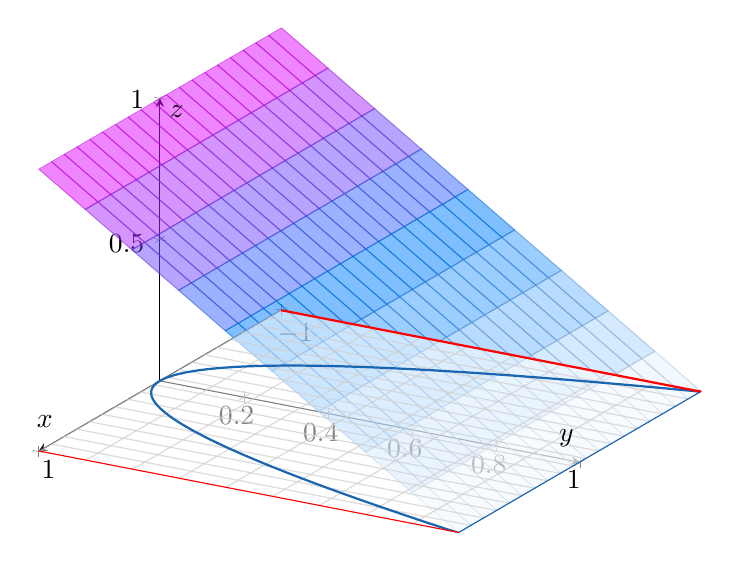
\begin{tikzpicture}
            \begin{axis}[
                    axis lines = middle,
                    xlabel = $x$,
                    ylabel = $y$,
                    zlabel = $z$,
                    domain=-1:1,
                    y domain=0:1,
                    samples=20,
                    samples y=10,
                    colormap/cool,
                    view={120}{30},
                    width=10cm,
                    height=8cm,
                ]
                % Draw the surface z = 1 - y
                \addplot3[surf, opacity=0.5] {1 - y};
                % Draw the plane z = 0
                \addplot3[surf, opacity=0.5] {0};
                % Draw the curve y = x^2
                \addplot3[domain=-1:1, samples=100, thick, blue] ({x}, {x^2}, {0});
                % Draw the vertical lines at x = -1 and x = 1
                \addplot3[domain=0:1, samples=100, thick, red] ({-1}, {x}, {0});
                \addplot3[domain=0:1, samples=100, thick, red] ({1}, {x}, {0});
            \end{axis}
        \end{tikzpicture}
        \caption{The region bounded by $z = 1 - y$, $z = 0$, $y = x^2$, $x = -1$, and $x = 1$.}
    \end{figure}
    
    
    We can also visualize the $R$ that is the reigion projected in the $xy$-plane as follows
    
    \begin{figure}[h!]
        \centering
        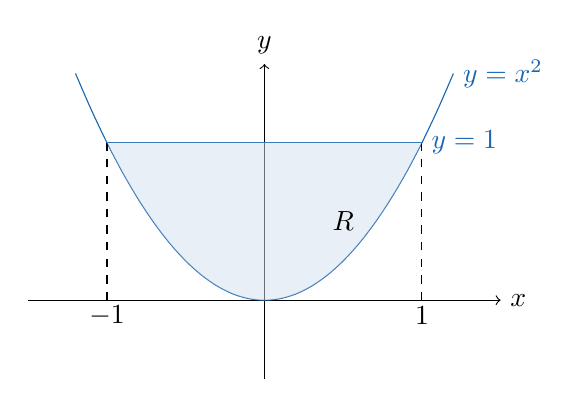
\begin{tikzpicture}[scale=2]
            % Draw axes
            \draw[->] (-1.5,0) -- (1.5,0) node[right] {$x$};
            \draw[->] (0,-0.5) -- (0,1.5) node[above] {$y$};
            
            % Draw the curve y = x^2
            \draw[domain=-1.2:1.2,smooth,variable=\x,blue] plot ({\x},{\x*\x}) node[right] {$y = x^2$};
            % Draw the line y = 1
            \draw[blue] (-1,1) -- (1,1) node[right] {$y = 1$};

            %vertical labels for x = pm1
            \draw[dashed] (-1,0) -- (-1,1);
            \draw[dashed] (1,0) -- (1,1);
            \node at (-1,-0.1) {$-1$};
            \node at (1,-0.1) {$1$};

            % Shade the region
            \fill[blue!20,opacity=0.5] plot[domain=-1:1,smooth,variable=\x] ({\x},{\x*\x}) -- (1,1) -- (-1,1) -- cycle;
            % Add labels
            \node at (0.5,0.5) {$R$};
        \end{tikzpicture}
        \caption{The projection of the region onto the $xy$-plane.}
        
    \end{figure}

    So, we can consider the projection of the triangle on the $zy$-plane as our base region $R'$. Then, we consider how the region changes in the $x$ direction over $R$:
    $$
        x^2 = y \implies -\sqrt{y} \le x \le \sqrt{y}
    $$
    So we can set up:
    \begin{align*}
        \iiint_V f(x,y,z) \, dV &= \iint_{R'} \int_{-\sqrt{y}}^{\sqrt{y}} f(x,y,z) \, dx \, dA \\
        &= \iint_{R'} \int_{-\sqrt{y}}^{\sqrt{y}} f(x,y,z) \, dx \, dy \, dz
    \end{align*}
    Now, we consider how the projection $R'$ change in the $y$ direction over $z$:
    $$        z = 1 - y \implies 0 \le y \le 1 - z, \quad 0 \le z \le 1
    $$
    So we can set up:
    \begin{align*}
        \iiint_V f(x,y,z) \, dV &= \int_0^1 \int_0^{1 - z} \int_{-\sqrt{y}}^{\sqrt{y}} f(x,y,z) \, dx \, dy \, dz
    \end{align*}
\end{example}
\subsubsection{Applications of Triple Integrals}
\paragraph{Physical Applications} Similar to double integrals, triple integrals can be used to compute physical quantities such as mass, center of mass, and moment of inertia for three-dimensional objects with variable density. 
\begin{definition}[Mass of a Solid]
    Consider a solid $V$ with a variable density function $\rho(x,y,z)$ that is continuous over the solid. The mass $M$ of the solid can be computed using the following triple integral:
    \begin{equation}
        M = \iiint_V \rho(x,y,z) \, dV
    \end{equation}
    
\end{definition}

\begin{definition}[Center of Mass of a Solid]
    Consider a solid $V$ with a variable density function $\rho(x,y,z)$ that is continuous over the solid. The coordinates of the center of mass $(\bar{x}, \bar{y}, \bar{z})$ of the solid can be computed using the following formulas:
    \begin{equation}
        \bar{x} = \frac{1}{M} \iiint_V x \rho(x,y,z) \, dV, \quad \bar{y} = \frac{1}{M} \iiint_V y \rho(x,y,z) \, dV, \quad \bar{z} = \frac{1}{M} \iiint_V z \rho(x,y,z) \, dV
    \end{equation}
    where $M$ is the mass of the solid.
    
\end{definition}


\begin{definition}[Moment of Inertia of a Solid]
    Consider a solid $V$ with a variable density function $\rho(x,y,z)$ that is continuous over the solid. The moment of inertia of the solid about the $x$-axis ($I_x$), $y$-axis ($I_y$), and $z$-axis ($I_z$) can be computed using the following formulas:
    \begin{equation}
        I_x = \iiint_V (y^2 + z^2) \rho(x,y,z) \, dV, \quad I_y = \iiint_V (x^2 + z^2) \rho(x,y,z) \, dV, \quad I_z = \iiint_V (x^2 + y^2) \rho(x,y,z) \, dV
    \end{equation}
    where $y^2 + z^2$, $x^2 + z^2$, and $x^2 + y^2$ are the squares of the distances from the respective axes of rotation, and $\rho(x,y,z) \, dV$ represents the mass element of the solid at the point $(x,y,z)$.

    Also for the moment of inertia about the origin ($I_o$):
    \begin{equation}
        I_o = \iiint_V (x^2 + y^2 + z^2) \rho(x,y,z) \, dV
    \end{equation}
    In general, for an axis defined by a line $ax + by + cz + d = 0$, the moment of inertia about that axis ($I_l$) can be found using the following formula:
    \begin{equation}
        I_l = \iiint_V \left( \frac{ax + by + cz + d}{\sqrt{a^2 + b^2 + c^2}} \right)^2 \rho(x,y,z) \, dV
    \end{equation}
\end{definition}

\begin{example}
    \textit{Find the center of mass of a solid of constant density $\rho_0$ that is bounded by the parabolic cylinder $x = y^2$ and the planes $z=0$, $x=z$ and $x=1$.}
    We visualize the solid as follows:
    \begin{figure}[h!]
        \centering
        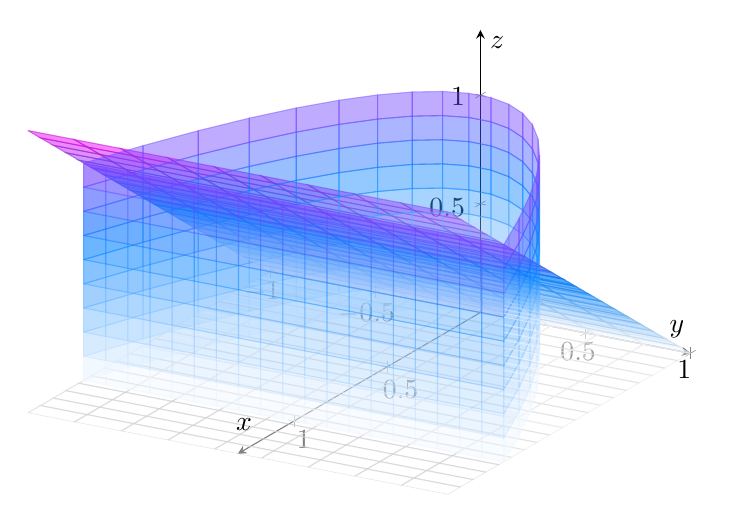
\begin{tikzpicture}
            \begin{axis}[
                    axis lines = middle,
                    xlabel = $x$,
                    ylabel = $y$,
                    zlabel = $z$,
                    domain=0:1.3,
                    y domain=-1:1,
                    samples=20,
                    samples y=10,
                    colormap/cool,
                    view={120}{30},
                    width=10cm,
                    height=8cm,
                ]
                % Draw the surface z = x
                \addplot3[surf, opacity=0.5] {x};
                % Draw the plane z = 0
                \addplot3[surf, opacity=0.5] {0};

                % Draw the surface cylinder x = y^2 on the plane z = 0, and it extends to z = x
                % Parabolic cylinder x = y^2 (y in [-1,1], z in [0,1])
                \addplot3[surf, opacity=0.45, shader=flat, domain=-1:1, y domain=0:1] ({x^2}, {x}, {y});
                % bottom z = 0
                \addplot3[surf, opacity=0.25, shader=flat, domain=0:1, y domain=-1:1] ({x}, {y}, {0});
                % slanted plane x = z (i.e. z = x)
                \addplot3[surf, opacity=0.35, shader=flat, domain=0:1, y domain=-1:1] ({x}, {y}, {x});
                % vertical plane x = 1 (closes the solid)
                \addplot3[surf, opacity=0.30, shader=flat, domain=-1:1, y domain=0:1] ({1}, {x}, {y});
                % fill the surface such that
            \end{axis}
        \end{tikzpicture}
        \caption{The solid bounded by the surfaces $x = y^2$, $z = 0$, $x = z$, and $x = 1$.}
    \end{figure}
    We can find the mass of the solid:
    \begin{align*}
        M &= \iiint_V \rho_0 \, dV = \rho_0 \iiint_V 1 \, dV \\
        &= \rho_0 \int_{-1}^1 \int_{y^2}^1 \int_{0}^x 1 \, dz \, dx \, dy \\
        &= \rho_0 \cdot \frac{4}{5}
    \end{align*}

    Next, we can find the coordinates of the center of mass:
    \begin{align*}
        \bar{x} &= \frac{1}{M} \iiint_V x \rho_0 \, dV = \frac{\rho_0}{M} \iiint_V x \, dV = 5/7 \\
        \bar{y} &= \frac{1}{M} \iiint_V y \rho_0 \, dV = \frac{\rho_0}{M} \iiint_V y \, dV = 0 \text{ (by symmetry)} \\
        \bar{z} &= \frac{1}{M} \iiint_V z \rho_0 \, dV = \frac{\rho_0}{M} \iiint_V z \, dV = 5/14 \\
    \end{align*}    
\end{example}

\begin{example}
    \textit{Find the moment of inertia of a cyliner with radius $a$ and height $h$ about its central axis, assuming the cylinder has a constant density $\rho_0$.}
    We consider the base region $R$ as the circular base of the cylinder in the $xy$-plane. Then, we consider how the cylinder change in the $z$ direction over $R$:
    $$
        0 \le z \le h
    $$
    So we can set up:
    \begin{align*}
        I_z &= \iiint_V (x^2 + y^2) \rho_0 \, dV = \rho_0 \iint_R \int_0^h (x^2 + y^2) \, dz \, dA \\
        &= \rho_0 h \iint_R (x^2 + y^2) \, dA
    \end{align*}

    Then, we can express the base region $R$ in polar coordinates:
    $$        
    x^2 + y^2 = r^2 \implies 0 \le r \le a, \quad 0 \le \theta \le 2\pi
    $$
    So we can set up:
    \begin{align*}
        I_z &= \rho_0 h \int_0^{2\pi} \int_0^a r^2 \cdot r \, dr \, d\theta \\
        &= \rho_0 h \int_0^{2\pi} \left[ \frac{r^4}{4} \right]_{r=0}^{r=a} \, d\theta = \frac{\pi \rho_0 h a^4}{2}
    \end{align*}
    This also leads to the well-known formula for the moment of inertia of a solid cylinder about its central axis:
    $$
        I_z = \frac{1}{2} M a^2
    $$
    where $M = \pi a^2 h \rho_0$ is the mass of the cylinder. 
\end{example}
\subsection{Triple Integrals in Cylindrical Coordinates}
\begin{definition}[Cylindrical Coordinates]
    The cylindrical coordinates of a point $P$ in 3-D space are given by the ordered triple $(r, \theta, z)$, where:
    \begin{itemize}
        \item $r$ is the distance from the $z$-axis to the projection of $P$ onto the $xy$-plane,
        \item $\theta$ is the angle between the positive $x$-axis and the line segment from the origin to the projection of $P$ onto the $xy$-plane,
        \item $z$ is the same as in rectangular coordinates, representing the height of point $P$ above the $xy$-plane.
    \end{itemize}
    The relationships between cylindrical coordinates and rectangular coordinates are given by:
    \begin{equation}
        x = r \cos \theta, \quad y = r \sin \theta, \quad z = z
    \end{equation}
    and conversely:
    \begin{equation}
        r = \sqrt{x^2 + y^2}, \quad \theta = \tan^{-1}\left(\frac{y}{x}\right), \quad z = z
    \end{equation}

    For the change of variables in triple integrals, the volume element $dV$ in cylindrical coordinates is given by:
    \begin{equation}
        dV = dA \, dz = r \, dr \, d\theta \, dz
    \end{equation}
\end{definition}

\begin{example}
    Consider the triple integral in the cononical reigion $V$ bounded by the cone $z = \sqrt{x^2 + y^2}$ and the plane $z=2$. Changing to cylindrical coordinates, we consider the projection of the cone onto the $xy$-plane as our polar base region $R$. Then, we consider how the cone change in the $z$ direction over $R$:
    $$
        z = r \implies r \le z \le 2
    $$
    So the region $V_{\text{polar}}$ is:
    $$
    V_{\text{polar}} = \{(r, \theta, z) \mid 0 \le r \le 2, 0 \le \theta \le 2\pi, r \le z \le 2\}
    $$
    So we can set up:
    $$
        \iiint_V f(x,y,z) \, dV = \int_0^{2\pi} \int_0^2 \int_r^2 f(r \cos \theta, r \sin \theta, z) \, r \, dz \, dr \, d\theta
    $$

    Let $f(x,y,z) = x^2 +. y^2 = r^2$. Then, we have:
    \begin{align*}
        \iiint_V (x^2 + y^2) \, dV &= \int_0^{2\pi} \int_0^2 \int_r^2 r^2 \cdot r \, dz \, dr \, d\theta \\
        &= \int_0^{2\pi} \int_0^2 r^3 (2 - r) \, dr \, d\theta = \frac{16\pi}{5}
    \end{align*}

\end{example}
\subsection{Triple Integrals in Spherical Coordinates}
\begin{definition}[Spherical Coordinates]
    The spherical coordinates of a point $P$ in 3-D space are given by the ordered triple $(\rho, \phi, \theta)$, where:
    \begin{itemize}
        \item $\rho$ is the distance from the origin to the point $P$,
        \item $\phi$ is the angle between the positive $z$-axis and the line segment from the origin to point $P$ (also known as the polar angle or colatitude),
        \item $\theta$ is the angle between the positive $x$-axis and the projection of the line segment from the origin to point $P$ onto the $xy$-plane (also known as the azimuthal angle).
    \end{itemize}
    The relationships between spherical coordinates and rectangular coordinates are given by:
    \begin{equation}
        x = \rho \sin \phi \cos \theta, \quad y = \rho \sin \phi \sin \theta, \quad z = \rho \cos \phi
    \end{equation}
    and conversely:
    \begin{equation}
        \rho = \sqrt{x^2 + y^2 + z^2}, \quad \phi = \cos^{-1}\left(\frac{z}{\sqrt{x^2 + y^2 + z^2}}\right), \quad \theta = \tan^{-1}\left(\frac{y}{x}\right)
    \end{equation}

    For the change of variables in triple integrals, the volume element $dV$ in spherical coordinates is given by:
    \begin{equation}
        dV = \rho^2 \sin \phi \, d\rho \, d\phi \, d\theta
    \end{equation}
\end{definition}

\begin{example}
    \textit{find the mass of a half sphere of radius $a$ that has a density $ k(2a - \rho)$, where $k$ is a constant and $\rho$ is the distance from the origin.}

    Let $\lambda = k(2a - \rho)$ be the density function. Then, we consider the half sphere $S$ in spherical coordinates:
    $$       
    S = \{(\rho, \phi, \theta) \mid 0 \le \rho \le a, 0 \le \phi \le \frac{\pi}{2}, 0 \le \theta \le 2\pi\}
    $$
    So we can set up:
    \begin{align*}
        M &= \iiint_S \lambda \, dV = \iiint_S k(2a - \rho) \, dV \\
        &= k \int_0^{2\pi} \int_0^{\frac{\pi}{2}} \int_0^a (2a - \rho) \rho^2 \sin \phi \, d\rho \, d\phi \, d\theta \\
        &= k \int_0^{2\pi} \int_0^{\frac{\pi}{2}} \left[ 2a \cdot \frac{\rho^3}{3} - \frac{\rho^4}{4} \right]_{\rho=0}^{\rho=a} \sin \phi \, d\phi \, d\theta \\
        &= k \int_0^{2\pi} \int_0^{\frac{\pi}{2}} \left( \frac{2a^4}{3} - \frac{a^4}{4} \right) \sin \phi \, d\phi \, d\theta \\
        &= k \cdot \frac{5a^4}{12} \int_0^{2\pi} \left[ -\cos \phi \right]_{\phi=0}^{\phi=\frac{\pi}{2}} \, d\theta = k \cdot \frac{5a^4}{12} \cdot 2\pi \\ 
        &= \frac{5\pi k a^4}{6}
    \end{align*}

\end{example}

\subsection{}
\subsection{Change of Variables in Multiple Integrals} \label{sec:change_of_variables}
\chapter{Fluid Mechanics}
\end{document} 